%!TeX root = main.tex
\chapter{Operationen auf meromorphen Zusammenhängen}
\section{Tensorprodukt}
\begin{comment}
\begin{defn}[Tensorprodukt]
\cite[3(Algebra).11.21]{stacks-project}
% von Vorlesung Algebra 2
\begin{center}
\begin{tikzpicture} [scale=3.3, descr/.style={fill=white,inner sep=2.5pt} ]
  \matrix (m) [
    matrix of math nodes
    , row sep=2em
    , column sep=3em
    %, text height=3em
    %, text depth=0.25em
  ]{
    M\times N & M\otimes_RN \\
              & T \\
  };
  %TODO: Pfeile
  \path[->,font=\scriptsize,>=angle 90]
  (m-1-1) edge node[above]{$  $} (m-1-2)
  (m-1-1) edge node[below]{$f$} (m-2-2)
  ;
  \path[->,font=\scriptsize,>=angle 90,dashed]
  (m-1-2) edge node[right]{$\exists!\gamma$} (m-2-2)
  ;
\end{tikzpicture}
\end{center}
Für eine Abbildung $f:M\rightarrow M'$ definiere das Tensorprodukt davon über
$R$ mit $N$ als
\[
\id_N \otimes f:
\begin{array}[t]{ccc}
N\otimes_{R}M & \rightarrow & N\otimes_{R}M'\\
n\otimes m & \mapsto & n\otimes f(m)
\end{array}
\]
\end{defn}
\end{comment}
\begin{bem} \label{bem:Rechenregeln-Tensorprodukt}
Hier einige Rechenregeln für das Tensorprodukt,
\begin{align}
(M\otimes_R N)\otimes_S L &\cong M\otimes_R (N \otimes_S L)
  \label{bem:Rechenregeln-Tensorprodukt1}\\
M\otimes_R R &\cong M \label{bem:Rechenregeln-Tensorprodukt2}
\end{align}
Sei $f:M'\rightarrow M$ eine Abbildung, so gilt
\begin{align}
N\otimes_R(M/\im(f)) &\cong N\otimes_R M / \im(\id_{R}\otimes f)
\label{bem:Rechenregeln-Tensorprodukt3}
\end{align}
\end{bem}

\begin{prop} \label{prop:tensorZusammenhang}
Seien $(\cM,\partial_\cM)$ und $(\cN,\partial_\cN)$ meromorphe Zusammenhänge.
Sei $n\otimes n\in \cM\otimes_K\cN$.
Durch Setzten von
\begin{equation} \label{eq:TensorAbleiten}
\partial_\otimes(m\otimes n)=\partial_\cM(m)\otimes n +m\otimes \partial_\cN(n)
\end{equation}
als die Wirkung von $\partial$ auf das $K$-Modul $\cM\otimes_K\cN$, wird
$(\cM\otimes_K\cN,\partial)$ zu einem meromorphen Zusammenhang.
\begin{comment}
\cite[Prop 4.1.1]{SchneidersDmod}
\end{comment}
\end{prop}
\begin{comment}
TODO: Zeige universelle Eigenschaft
\end{comment}
\begin{comment}
\begin{proof}
Klar
\end{proof}
\end{comment}
\begin{lem} 
%TODO: move after slope definition!!!
Falls $\cN$ regulär und nicht Null, dann ist die Menge der Slopes von
$\cM\otimes\cN$ genau die Menge der Slopes von $\cM$.
\end{lem}
\begin{proof}
Siehe \cite[Ex 5.3.7]{sabbah_cimpa90}.
\begin{comment}
TODO
\end{comment}
\end{proof}

\section{pull-back und push-forward}
\begin{comment}
Nach \cite[1.a]{sabbah_Fourier-local} und \cite[1.3]{hotta2007d}.
\end{comment}
Es sei
\begin{align*}
\rho&:\C\rightarrow \C , t\mapsto x:=\rho(t) &\in t\Cft
\end{align*}
eine polynomielle Abbildung mit  Bewertung $p\geq1$.
Hier werden wir meistens $\rho(t)=t^p$ für ein $p\in \N$ betrachten. Diese
Funktion induziert eine Abbildung
\begin{align*}
\rho^*&:\Ckx\hookrightarrow \Ckt, f \mapsto f\circ \rho & \mbox{bzw.} &&
\rho^*&:\Cfx\hookrightarrow \Cft, f \mapsto f\circ \rho \,.
\end{align*}
Analog erhalten wir
\begin{align*}
\rho^*&:K\hookrightarrow L:=\Cktl, f \mapsto f\circ \rho & \mbox{bzw.} &&
\rho^*&:\hat K\hookrightarrow \hat L:=\Cftl, f \mapsto f\circ \rho \,,
\end{align*}
wobei $L$ (bzw. $\hat L$) eine endliche Körpererweiterung von $K$ (bzw. $\hat
K$) ist.
\begin{comment}
TODO: damit wird $\hat L$ zu einem $\hat K$ Vektorraum.
\end{comment}
\begin{comment}
TODO: $\nable$ zu $\partial_x$ ???? dann $\partial_t=\rho^*\partial_x$???
\end{comment}
Sei $\cM_{\hat K}$ ein endlich dimensionaler $\Cfxl$ Vektorraum ausgestattet mit
einem Zusammenhang $\nabla$.
%
\begin{defn}[pull-back] \label{defn:pull-back}
\begin{comment}
\cite[1.a]{sabbah_Fourier-local} und
\cite[Page 34]{sabbah_cimpa90}
\end{comment}
Der \emph{pull-back} oder das \emph{inverse Bild} $\rho^{+}\cM_{\hat K}$ von
$(\cM_{\hat K},\nabla)$ ist der Vektorraum
\[
\rho^{*}\cM_{\hat K}:=\hat L\otimes_{\hat K}\cM_{\hat K}
\bydef\Cftl\otimes_{\Cfxl}\cM_{\Cfxl}
\]
 mit dem \emph{pull-back Zusammenhang} $\rho^*\nabla$ definiert durch
%TODO: ist das der Zusammenhang oder die Wirkung oder was?
\begin{equation} \label{eq:pull-back-zusammenhang}
\partial_t(1\otimes m):=\rho'(t)\otimes\partial_xm \,.
\end{equation}
\end{defn}
Für ein allgemeines $\phi\otimes m\in \rho^{*}\cM_{\hat K}$ gilt somit
\begin{equation} \label{eq:pull-back-zusammenhang-2}
\partial_t(\phi\otimes m):=\rho'(t)(\phi\otimes\partial_xm) +
  \frac{\partial\phi}{\partial t}\otimes m \,.
\end{equation}
\begin{comment}
Nun wollen wir uns noch genauer mit dem pull-back beschäftigen, und stellen uns
die Frage:
\paragraph{Wie sieht die Wirkung der Derivation auf dem pull-back Zusammenhang
aus?} Für $\rho(t)=t^p$ betrachten wir beispielsweise ein Element der Form
$f(x)m=f(\rho(t))m\in\rho^*\cM_{\hat K}$, dann gilt
\begin{align*}
\partial_x(f(x)m) &= \partial_{\rho(t)}(f(\rho(t))m) \\
  &= f'(\rho(t))\cdot \underset{=1}
  {\underbrace{\frac{\partial(f(t))}{\partial(f(t))}}}m +
  f(\rho(t))\underset{=\partial_x} {\underbrace{\partial_{\rho(t)}}}m
\\&= f'(\rho(t))m + f(\rho(t))\partial_x m
  = (\star)
\\ \rho'(t)^{-1}\partial_t(f(x)m) &= \frac{1}{pt^{p-1}}\partial_t(f(t^p)m)
\\ &= f'(t^p)m+f(t^p)\frac{1}{pt^{p-1}}\partial_t m = (\star) \\
\end{align*}
Also gilt $\partial_t(f(t)m) = \rho'(u)^{-1}\partial_u(f(t)m)$ und somit
lässt sich vermuten, dass die Wirkung von $\partial_x$ gleich der Wirkung von
$\rho'(t)^{-1}\partial_t$ ist. In der Tat stimmt diese Vermutung, wie das
folgende Lemma zeigt.
\end{comment}
\begin{comment}
Sei $f(x)m=f(\rho(t))m\in\rho^*\cM_{\hat K}$. Es gilt, dass
\begin{align*}
\partial_x(f(x)m) &= \partial_{\rho(t)}(f(\rho(t))m) \\
  &= f'(\rho(t))\cdot \underset{=1}
  {\underbrace{\frac{\partial(f(t))}{\partial(f(t))}}}m +
  f(\rho(t))\underset{=\partial_x} {\underbrace{\partial_{\rho(t)}}}m
\\&= f'(\rho(t))m + f(\rho(t))\partial_x m
\\&= f'(t^p)m+f(t^p)\frac{1}{pt^{p-1}}\partial_t m
\\&= \myubracket{\frac{1}{pt^{p-1}}}\partial_t(f(\myubracket{t^p})m)
\\&=\myobracket{\rho'(t)^{-1}}\partial_t(f(\myobracket{x})m) 
\end{align*}
und damit lässt sich vermuten, dass die Wirkung von $\partial_x$ genau die
Wirkung von $\rho'(t)^{-1}\partial_t$ ist. In der Tat ist dies, nach dem
folgenden Satz, wahr.
\end{comment}

Der folgende Satz zeigt, wie man mit dem pull-back rechnen lässt, bzw.
wie man konkret ein entsprechendes Minimalpolynom berechnen kann.
\begin{thm} \label{thm:pull-back-berechnung}
%Wie erhält man den pull-back Zusammenhang bzw. wie ist er berechenbar?
In der Situation von Lemma \ref{defn:pull-back}, mit
$\cM_{\hat K}=\cD_{\hat K}/\cD_{\hat K}\cdot P(x,\partial_x)$ für ein
$P(x,\partial_x)\in\cD_{\hat K}$, gilt
\[\rho^*\cM_{\hat K}\cong \cD_{\hat L}\Big/\cD_{\hat L}\cdot
  P(\rho(t),\rho'(t)^{-1}\partial_t) \,. \]
Für $P(\rho(t),\rho'(t)^{-1}\partial_t)$ werden wir auch
$\rho^*P(t,\partial_t)$ schreiben.
\end{thm}
\begin{comment}
\cite[Seite 130]{coutinho1995primer} Holonomic modules are preserved under
this construction.
\end{comment}
%
\begin{comment}
\cite[Page 34]{sabbah_cimpa90}
Sei $\cM_{\hat K}$ ein formaler meromorpher Zusammenhang. Man definiert
$\pi^*\cM_{\hat K}$ als den Vektor Raum über $\hat L:\pi^*\cM_{\hat K}=\hat
L\otimes_{\hat K}\cM_{\hat K}$. Dann definiert man die Wirkung von $\partial_t$
durch: $t\partial_t\cdot(1\otimes m)=q(1\otimes(x\partial_x\otimes m))$ und
damit
\[
t\partial_t\cdot(\phi\otimes m)=q(\phi\otimes(x\partial_x\cdot
m))+((t\frac{\partial\phi}{\partial t})\otimes m) \,.
\]
Man erhält damit die Wirkung von $\partial_t=t^{-1}(t\partial_t)$.
\end{comment}

Für den Beweis von Satz \ref{thm:pull-back-berechnung} werden zunächst einige
Lemmata bewiesen.

\begin{lem} \label{lem:pull-back-hilfslemma1pre}
Es gilt $\rho^*\cD_{\hat K }\bydef\hat L\otimes_{\hat K}\cD_{\hat K } \cong
\cD_{\hat L }$ als $\cD_{\hat L}$-Vektorräume, mittels
\begin{comment} TODO: VR oder Moduln??  \end{comment}
\begin{center}
\begin{tikzpicture} [scale=3.3, descr/.style={fill=white,inner sep=2.5pt} ]
\matrix (m) [
  matrix of math nodes
  %, row sep=1.5em
  , column sep=3em
  %, text height=3em
  %, text depth=0.25em
]{
  \Phi:\hat L\otimes_{\hat K}\cD_{\hat K }  & \cD_{\hat L } \\
  %1\otimes m(t,\partial_t) & m(\rho(u),\rho'(u)^{-1}\partial_u) \\
  %f(u)\otimes m(t,\partial_t) & f(u)m(\rho(u),\rho'(u)^{-1}\partial_u) \\
  f(t)\otimes Q(x,\partial_x) & f(t)Q(\rho(t),\rho'(t)^{-1}\partial_t) \\
};
%TODO: Pfeile
\path[->,font=\scriptsize,>=angle 90]
(m-1-1) edge node[above]{$\cong$} (m-1-2)
;
\path[|->,font=\scriptsize,>=angle 90]
(m-2-1) edge (m-2-2)
%(m-3-1) edge (m-3-2)
;
\end{tikzpicture}
\end{center}
\end{lem}
\begin{comment}
\begin{proof}
Wir wollen zeigen, dass $\cD_{\hat L}$ die universelle Eigenschaft für das
Tensorprodukt $\hat L\otimes_{\hat K}\cD_{\hat K }$ erfüllt, in diesem Fall
folgt die Behauptung. Zunächst sei die bilineare Abbildung
\[
\kappa: \hat
L\times\cD_{\hat K }\rightarrow\cD_{\hat L},\, (f(t),Q(x,\partial_x))\mapsto
f(t)Q(\rho(t),\rho'(t)^{-1}\partial_t)
\]
gegeben, und nach der universellen Eigenschaft des Tensorproduktes gibt es
genau eine lineare Abbildung, so dass das folgende Diagramm kommutiert.
\begin{center}
\begin{tikzpicture} [scale=3.3, descr/.style={fill=white,inner sep=2.5pt} ]
\matrix (m) [
  matrix of math nodes
  , row sep=3em
  , column sep=3em
  %, text height=3em
  %, text depth=0.25em
]{
  \hat L\times\cD_{\hat K } & \hat L\otimes_{\hat K}\cD_{\hat K }\\
  & \cD_{\hat L } \\
};
\path[->,font=\scriptsize,>=angle 90]
(m-1-1) edge node[above]{$\otimes$} (m-1-2)
        edge node[above]{$\kappa$} (m-2-2)
;
\path[->,dashed]
(m-1-2) edge node[right]{$\exists!$} (m-2-2)
;
\end{tikzpicture}
\end{center}
Dieser so erhaltene eindeutige Morphismus ist genau unser $\Phi$.
\begin{center}
\begin{tikzpicture} [scale=3.3, descr/.style={fill=white,inner sep=2.5pt} ]
\matrix (m) [
  matrix of math nodes
  , row sep=3em
  , column sep=3em
  %, text height=3em
  %, text depth=0.25em
]{
  \hat L\times\cD_{\hat K } & \hat L\otimes_{\hat K}\cD_{\hat K }\\
  & \cD_{\hat L } \\
  & V \\
};
\path[->,font=\scriptsize,>=angle 90]
(m-1-2) edge node[right]{$\Phi$} (m-2-2)
(m-1-1) edge node[above]{$\otimes$} (m-1-2)
        edge node[above]{$\kappa$} (m-2-2)
        edge node[above]{$\gamma$} (m-3-2)
;
\path[->,dashed,bend left=60]
(m-1-2) edge node[right]{$\exists!$} (m-3-2)
;
\path[->,dashed]
(m-2-2) edge node[right]{$\exists?$} (m-3-2)
;
\end{tikzpicture}
\end{center}
\end{proof}
\end{comment}
\begin{proof}
Prüfe zunächst die Injektivität. Sei $f(t)\otimes Q(x,\partial_x)\in
\ker(\Phi)$\footnote{
$\ker(\Phi):=\{x\in \hat L\otimes_{\hat K }\cD_{\hat K }\mid \Phi(x)=0\}$
} so, dass
\begin{align*}
0 &= \Phi(f(t)\otimes Q(x,\partial_x))
\\&= f(t)Q(\rho(t),\rho'(t)^{-1}\partial_t)
\end{align*}
und, da hier alles nullteilerfrei ist, ist die Bedingung äquivalent zur
folgenden
\begin{align*}
\Leftrightarrow && 0&=f(t) &\text{oder}&& 0&=Q(\rho(t),\rho'(t)^{-1}\partial_t)
\\\Leftrightarrow && 0&=f(t) &\text{oder}&& 0&=Q(x,\partial_x)
\\\Leftrightarrow&& 0&=f(t)\otimes Q(x,\partial_x) \,.
\end{align*}
\begin{comment} TODO: korrekt? \end{comment}
Nun zur Surjektivität.
Sei $g(t,\partial_t)=\sum_ka_k(t)\partial_t^k\in\cD_{\hat L}$, so gilt
\begin{align*}
g(t,\partial_t)&=\sum_ka_k(t)\partial_t^k
\\&=\sum_ka_k(t)(\underset{=1}{\underbrace{\rho'(t)\rho'(t)^{-1}}})^k
  \partial_t^k
\\&=\sum_ka_k(t)\rho'(t)^k(\rho'(t)^{-1} \partial_t)^k
\end{align*}
und zerlege $a_k(t)\rho'(t)^k=\sum_{i=0}^{p-1}t^ia_{k,i}(t^p)$. Damit gilt dann
\begin{align*}
g(t,\partial_t)&= \sum_k\sum_{i=0}^{p-1}t^ia_{k,i}(t^p)
  (\rho'(t)^{-1} \partial_t)^k
\\&= \sum_{i=0}^{p-1}t^i\Big(\sum_ka_{k,i}(t^p)
  (\rho'(t)^{-1} \partial_t)^k\Big)
\\&= \Phi\Big(\sum_{i=0}^{p-1}t^i\otimes(\sum_ka_{k,i}(x)
  (\partial_x)^k)\Big) \,.
\end{align*}
Somit haben wir ein Urbild gefunden und die Surjektivität gezeigt.
\end{proof}

\begin{lem} \label{lem:pull-back-hilfslemma1}
Das in Lemma \ref{lem:pull-back-hilfslemma1pre} definierte $\Phi$ ist sogar ein
Morphismus von meromorphen Zusammenhängen, also gilt sogar
$\rho^*\cD_{\hat K }\bydef\hat L\otimes_{\hat K}\cD_{\hat K } \cong \cD_{\hat L
}$
als meromorphe Zusammenhänge.
\end{lem}
\begin{proof}
Sei $\partial_t$ wie gewohnt und $\partial_\otimes$ der Zusammenhang auf
$\hat L\otimes_{\hat K}\cD_{\hat K }$, welcher wie in Proposition
\ref{prop:tensorZusammenhang} definiert sei.
Wir wollen noch zeigen, dass $\partial_t\circ\Phi = \Phi \circ
\partial_\otimes$ gilt, also dass $\Phi$ ein Morphismus von meromorphen
Zusammenhängen ist. Betrachte dazu das Diagramm
\begin{center}
\begin{tikzpicture} [scale=3.3, descr/.style={fill=white,inner sep=2.5pt} ]
\matrix (m) [
  matrix of math nodes
  , row sep=2.5em
  , column sep=5em
  %, text height=3em
  %, text depth=0.25em
]{
\hat L\otimes_{\hat K}\cD_{\hat K } & \hat L\otimes_{\hat K}\cD_{\hat K } \\
\cD_{\hat L } & \cD_{\hat L }\\
};
\path[->,font=\scriptsize,>=angle 90]
(m-1-1) edge node[above]{$\partial_\otimes$} (m-1-2)
(m-1-1) edge node[descr]{$\cong$} node[right]{$\Phi$} (m-2-1)
(m-1-2) edge node[descr]{$\cong$} node[right]{$\Phi$} (m-2-2)
(m-2-1) edge node[above]{$\partial_t$} (m-2-2)
;
\end{tikzpicture}
\end{center}
und für einen Elementartensor $f(t)\otimes Q(x,\partial_x)\in\hat
L\otimes_{\hat K}\cD_{\hat K }$
\begin{comment}
Q wie in großen Beweis später, Namenskollision
\end{comment}
folgt dann
\begin{center}
\begin{tikzpicture} [scale=3.3, descr/.style={fill=white,inner sep=2.5pt} ]
\matrix (m) [
  matrix of math nodes
  , row sep=2.5em
  , column sep=2em
  %, text height=3em
  %, text depth=0.25em
]{
f(t)\otimes Q(x,\partial_x) &
  \partial_tf(t)\otimes Q(x,\partial_x)
  + \rho'(t)\otimes \partial_xQ(x,\partial_x)\\
& \partial_tf(t)Q(x,\partial_x)
  + \underset{=1}{\underbrace{\rho'(t)\cdot \rho'(t)^{-1}}}
  \partial_tQ(\rho(t),\rho'(t)^{-q}\partial_t)\\
f(t)Q(\rho(t),\rho'(t)^{-1}\partial_t) &  \partial_tf(t)Q(x,\partial_x)
  + \partial_tQ(\rho(t),\rho'(t)^{-q}\partial_t)\\
};
\path[|->,font=\scriptsize,>=angle 90]
(m-1-1) edge node[right]{$\Phi$} (m-3-1)
(m-1-1) edge node[above]{$\partial_\otimes$} (m-1-2)
(m-3-1) edge node[above]{$\partial_t$} (m-3-2)
(m-1-2) edge node[right]{$\Phi$} (m-2-2)
;
\path[bend right=90]
(m-3-2) edge node[descr]{$=$} (m-2-2)
;
\end{tikzpicture} , %TODO: hier wirklich ein Komma??
\end{center}
also kommutiert das Diagramm.
\end{proof}
\begin{comment}
\begin{bem}
BENÜTZT BEREITS DAS NÄCHSTE LEMMA...

Das soeben, in Lemma \ref{lem:pull-back-hilfslemma1pre}, definierte $\Phi$ erfüllt
für Elementartensoren $1\otimes m\in \hat L\otimes_{\hat K}\cD_{\hat K}$
\begin{align*}
\partial_u(1\otimes m) &\bydef \rho'(t)\otimes\partial_x m \\
&\overset{\Phi}{\mapsto} \underset{=1}{\underbrace{\rho'(t)\rho'(t)^{-1}}}
  \partial_t m(\rho(t),\rho'(t)^{-1}\partial_t) \\
&= \partial_t m(\rho(t),\rho'(t)^{-1}\partial_t)\\
&=\dots
\end{align*}
und somit (\ref{eq:pull-back-zusammenhang}) wie gewollt.
\end{bem}
\end{comment}
%
\begin{lem} \label{lem:pull-back-hilfslemma2}
Sei $P(x,\partial_x)\in \cD_K$. In der Situation
\begin{center}
\begin{tikzpicture} [scale=3.3, descr/.style={fill=white,inner sep=2.5pt} ]
\matrix (m) [
  matrix of math nodes
  , row sep=2.5em
  , column sep=5em
  %, text height=3em
  %, text depth=0.25em
]{
\hat L\otimes_{\hat K}\cD_{\hat K } & \hat L\otimes_{\hat K}\cD_{\hat K } \\
\cD_{\hat L } & \cD_{\hat L } \\
};
%TODO: Pfeile
%\path (m-1-1) edge[white] node{$\%$} (m-2-2);
\path[->,font=\scriptsize,>=angle 90]
(m-1-1) edge node[above]{$\id\otimes\_\!\cdot\! P(x,\partial_x)$} (m-1-2)
(m-1-1) edge node[descr]{$\cong$} node[right]{$\Phi$} (m-2-1)
(m-1-2) edge node[descr]{$\cong$} node[right]{$\Phi$} (m-2-2)
(m-2-1) edge node[above]{$\alpha$} (m-2-2)
;
\end{tikzpicture}
\end{center}
mit $\Phi$ wie in Lemma \ref{lem:pull-back-hilfslemma1pre}
macht $\alpha:=\_\!\cdot\! P(\rho(t),\rho'(t)^{-1}\partial_t)$ das Diagramm
kommutativ.
\end{lem}
\begin{proof}
Betrachte ein $f(t)\otimes Q(x,\partial_x)\in\hat L\otimes_{\hat K}\cD_{\hat
K}$. So gilt
\begin{center}
\begin{tikzpicture} [scale=3.3, descr/.style={fill=white,inner sep=2.5pt} ]
\matrix (m) [
  matrix of math nodes
  , row sep=2.5em
  , column sep=5em
  %, text height=3em
  %, text depth=0.25em
]{
f(t)\otimes Q(x,\partial_x) & f(t)\otimes Q(x,\partial_x)\cdot P(x,\partial_x)\\
& f(t) Q(\rho(t),\rho'(t)^{-1}\partial_t)
  \cdot P(\rho(t),\rho'(t)^{-1}\partial_t) \\
};
%TODO: Pfeile
%\path (m-1-1) edge[white] node{$\%$} (m-2-2);
\path[|->,font=\scriptsize,>=angle 90]
(m-1-1) edge node[above]{$\id\otimes\_\!\cdot\! P(x,\partial_x)$} (m-1-2)
(m-1-2) edge node[right]{$\Phi$} (m-2-2)
;
\end{tikzpicture}
\end{center}
und
\begin{center}
\begin{tikzpicture} [scale=3.3, descr/.style={fill=white,inner sep=2.5pt} ]
\matrix (m) [
  matrix of math nodes
  , row sep=2.5em
  , column sep=10em
  %, text height=3em
  %, text depth=0.25em
]{
f(t)\otimes Q(x,\partial_x) \\
f(t) Q(\rho(t),\rho'(t)^{-1}\partial_t) &
f(t) Q(\rho(t),\rho'(t)^{-1}\partial_t)
  \cdot P(\rho(t),\rho'(t)^{-1}\partial_t) \,, \\
};
%TODO: Pfeile
%\path (m-1-1) edge[white] node{$\%$} (m-2-2);
\path[|->,font=\scriptsize,>=angle 90]
(m-1-1) edge node[right]{$\Phi$} (m-2-1)
(m-2-1) edge node[above]{$\_\!\cdot\! P(\rho(t),\rho'(t)^{-1}\partial_t)$}
  (m-2-2)
;
\end{tikzpicture}
\end{center}
also kommutiert das Diagramm mit $\alpha=\_\!\cdot\!
P(\rho(t),\rho'(t)^{-1}\partial_t)$.
\end{proof}

\begin{proof}[Beweis zu Satz \ref{thm:pull-back-berechnung}]
%TODO: warum hier alles Lokalisiert?
Sei $P\in\cD_{\hat K}$ und $\cM_{\hat K }:=\cD_{\hat K }/\cD_{\hat K }\cdot P$.
Wir wollen zeigen, dass
\[
\rho^*\cM_{\hat K }\cong\cD_{\hat L }/\cD_{\hat L }\cdot Q
\]
für $Q=P(\rho(t),\rho'(t)^{-1}\partial_t)$ gilt.
Betrachte dazu die kurze Sequenz
\begin{center}
\begin{tikzpicture} [scale=3.3, descr/.style={fill=white,inner sep=2.5pt} ]
  \matrix (m) [
    matrix of math nodes
    %, row sep=2em
    , column sep=2.7em
    %, text height=3em
    %, text depth=0.25em
  ]{
  0 & \cD_{\hat K }    & \cD_{\hat K } & \cM_{\hat K }               & 0\\
    & \phantom{P}\!\!u & u\cdot P \\
    &                  & u             & u\mod\cD_{\hat K}\cdot P \\
  };
  \path[->,font=\scriptsize,>=angle 90]
  (m-1-1) edge (m-1-2)
  (m-1-2) edge node[above]{$\_\!\cdot\! P$} (m-1-3)
  (m-1-3) edge node[above]{$\pi_{\hat K}$} (m-1-4)
  (m-1-4) edge (m-1-5)
  ;
  \path[|->,font=\scriptsize,>=angle 90]
  (m-2-2) edge (m-2-3)
  (m-3-3) edge (m-3-4)
  ;
\end{tikzpicture}
\end{center}
ist exakt, weil $\cM_{\hat K } \cong\cD_{\hat K }\Big/\cD_{\hat K }\cdot
P=\coker(\_\cdot P)$.  Weil $\hat L$ flach über den Körper $\hat K$ ist, ist
auch, nach Anwenden des Funktors $\hat L\otimes_{\hat K}\_$, die Sequenz
%TODO: Funktorialität von Pull-Back? NEIN: Funktorialität von tensor
\begin{center}
\begin{tikzpicture} [scale=3.3, descr/.style={fill=white,inner sep=2.5pt} ]
  \matrix (m) [
    matrix of math nodes
    , row sep=-.5em
    , column sep=2.7em
    %, text height=3em
    %, text depth=0.25em
  ]{
  0 & \hat L\otimes_{\hat K}\cD_{\hat K}
    & \hat L\otimes_{\hat K}\cD_{\hat K}
    & \hat L\otimes_{\hat K}\cM_{\hat K}
    & 0\\
    & & & \shortparallel\\
    & & & \rho^*\cM_{\hat K} \\
  };
  %TODO: Pfeile
  \path[->,font=\scriptsize,>=angle 90]
  (m-1-1) edge (m-1-2)
  (m-1-2) edge node[above]{$\id\otimes\_\!\cdot\! P$} (m-1-3)
  (m-1-3) edge node[above]{$\id\otimes\pi_{\hat K}$} (m-1-4)
  (m-1-4) edge (m-1-5)
  ;
\end{tikzpicture}
\end{center}
exakt.
\begin{comment}
Deshalb ist
\begin{align*}
\rho^*\cM_{\hat K} &\cong \coker(\id\otimes\_\cdot P)
  & \mbox{(weil exakt)}\\
&\cong \hat L\otimes_{\hat K}\cD_{\hat K } \Big/
  \Big(( \hat L\otimes_{\hat K}\cD_{\hat K } )
  \cdot (\id\otimes\_\!\cdot\!  P) \Big)
  & \mbox{(nach def. von $\coker$)}
\end{align*}
\end{comment}
Also mit $\Phi$ wie in Lemma \ref{lem:pull-back-hilfslemma1pre} und
$Q(t,\partial_t):=P(\rho(t),\rho'(t)^{-1}\partial_t)$
nach Lemma \ref{lem:pull-back-hilfslemma2}
ergibt sich
\begin{center}
\begin{tikzpicture} [scale=3.3, descr/.style={fill=white,inner sep=2.5pt} ]
  \matrix (m) [
    matrix of math nodes
    , row sep=2em
    , column sep=2.7em
    %, text height=3em
    %, text depth=0.25em
  ]{
  0 & \hat L\otimes_{\hat K}\cD_{\hat K}
    & \hat L\otimes_{\hat K}\cD_{\hat K}
    & \rho^*\cM_{\hat K}
    & 0\\
 & \cD_{\hat L }
    & \cD_{\hat L }
    &
    & \\
  };
  %TODO: Pfeile
  \path[->,font=\scriptsize,>=angle 90]
  (m-1-1) edge (m-1-2)
  (m-1-2) edge node[above]{$\id\otimes\_\!\cdot\! P$} (m-1-3)
  (m-1-3) edge (m-1-4)
  (m-1-4) edge (m-1-5)

  (m-1-2) edge node[descr]{$\cong$} node[right]{$\Phi$} (m-2-2)
  (m-1-3) edge node[descr]{$\cong$} node[right]{$\Phi$} (m-2-3)

  (m-2-2) edge node[above]{$\_\!\cdot\! Q$} (m-2-3)
  ;
\end{tikzpicture}
\end{center}
als kommutatives Diagramm. Nun, da $\_\!\cdot\! Q$ injektiv ist, lässt sich
die untere Zeile zu einer exakten Sequenz fortsetzen
\begin{center}
\begin{tikzpicture} [scale=3.3, descr/.style={fill=white,inner sep=2.5pt} ]
  \matrix (m) [
    matrix of math nodes
    , row sep=2em
    , column sep=2.7em
    %, text height=3em
    %, text depth=0.25em
  ]{
  0 & \hat L\otimes_{\hat K}\cD_{\hat K}
    & \hat L\otimes_{\hat K}\cD_{\hat K}
    & \rho^*\cM_{\hat K}
    & 0\\
  0 & \cD_{\hat L }
    & \cD_{\hat L }
    & \cD_{\hat L }\Big/\cD_{\hat L }\cdot Q
    & 0 \\
  };
  %TODO: Pfeile
  \path[->,font=\scriptsize,>=angle 90]
  (m-1-1) edge (m-1-2)
  (m-1-2) edge node[above]{$\id\otimes\_\!\cdot\! P$} (m-1-3)
  (m-1-3) edge node[above]{$\id\otimes\pi_{\hat K}$} (m-1-4)
  (m-1-4) edge (m-1-5)

  (m-1-2) edge node[descr]{$\cong$} node[right]{$\Phi$} (m-2-2)
  (m-1-3) edge node[descr]{$\cong$} node[right]{$\Phi$} (m-2-3)
  %(m-1-4) edge[dashed,lightgray] node[right]{$\phi$} (m-2-4)

  (m-2-1) edge (m-2-2)
  (m-2-2) edge node[above]{$\_\!\cdot\! Q$} (m-2-3)
  (m-2-3) edge node[above]{$\pi_{\hat L}$} (m-2-4)
  (m-2-4) edge (m-2-5)
  ;
\end{tikzpicture}
\end{center}
und damit folgt, wegen Isomorphie der Kokerne, die Behauptung.
\end{proof}
%
\begin{lem}\label{lem:slope-pb-multiplikation}
Sei $\cP(\cM_{\hat K})=\{\Lambda_1,\dots,\Lambda_r\}$ die Menge der Slopes von
$\cM_{\hat K}$ und $\rho:t\mapsto x:=t^p$, dann gilt für $\cP(\rho^*\cM_{\hat
K})=\{\Lambda_1',\dots,\Lambda_r'\}$, dass $\Lambda_i'=p\cdot\Lambda_i$.
\end{lem}
\begin{proof}
Siehe \cite[5.4.3]{sabbah_cimpa90} für einen Beweis.
\end{proof}
\begin{comment}
\begin{proof}
Sei $\cM_{\hat K}=\cD_{\hat K}\slash \cD_{\hat K}\cdot P$ mit $P=\sum
a_i(x)\partial_x^i$, dann ist
$\rho^*\cM_{\hat K}\cong\cD_{\hat L}\slash \cD_{\hat L}\cdot P'$ mit
\begin{align*}
H(P'(t,\partial_t)) &=H(P(\rho(t),\rho'(t)^{-1}\partial_t))
\\&=H(\sum_i a_i(\rho(t))(\rho'(t)^{-1}\partial_t)^ii)
\\&=H(\sum_i a_i(\rho(t))(\rho'(t)^{-1}\partial_t)^ii)
\\&=H(\sum_i a_i(t^p)((p\cdot t^{p-1})^{-1}\partial_t)^i)
\\&=H(\sum_i a_i(t^p)(p\cdot t^{p-1})^{-i}\partial_t^i)
\\&=H(\sum_i a_i(t^p)t^{-i(p-1)}\partial_t^i)
\\&=\dots %TODO: Hier weiter...
\end{align*}
\end{proof}
\end{comment}
%
Hier nun ein explizit berechneter pull-back.
\begin{exmp}\label{exmp:Pull-Back}
Wir wollen $\cM_{\hat K}:=\cD_{\hat K}/\cD_{\hat K}\cdot P$ bzgl. $P:=
x^3\partial_x^2-4x^2\partial_x-1$ betrachten.
Unser Ziel ist es, hier ganzzahlige Slopes zu erhalten.
%TODO: erkläre wieso --> Elementare Zusammenhänge
Es gilt $\slopes(P)=\{\frac{1}{2}\}$ (siehe Abbildung \ref{fig:Pull-Back1}).
Wende den pull-back mit $\rho:t\rightarrow x:=t^2$ an.
Zunächst einige Nebenrechnungen, damit wir Satz
\ref{thm:pull-back-berechnung} einfacher anwenden können:
\begin{align*}
\partial_x   &\rightsquigarrow
  \frac{1}{\rho'(t)}\partial_t=\frac{1}{2t}\partial_t \,,
\\\partial_x^2 &\rightsquigarrow (\frac{1}{2t}\partial_t)^2
  = \frac{1}{2t}\partial_t (\frac{1}{2t}\partial_t)
  = \frac{1}{2t}(-\frac{1}{2t^2}\partial_t + \frac{1}{2t}\partial_t^2)
  = \frac{1}{4t^2}\partial_t^2-\frac{1}{4t^3}\partial_t \,.
\end{align*}
Also ergibt Einsetzen
\begin{align*}
\rho^*P &= (t^2)^3(\frac{1}{4t^2}\partial_t^2-\frac{1}{4t^3}\partial_t)-
    4(t^2)^2\frac{1}{2t}\partial_t-1
\\&= \frac{1}{4}t^4\partial_t^2 \myubracket{-t^3\frac{1}{4}\partial_t-
    4t^{3}\frac{1}{2}\partial_t}-1
\\&= \frac{1}{4}t^4\partial_t^2 \myobracket{-2\frac{1}{4}t^3\partial_t}-1 \,.
\end{align*}
%
Also ist $\rho^*P= \frac{1}{4}t^4\partial_t^2 -\frac{1}{2}t^3\partial_t-1$ mit
$ \slopes(\rho^*P)=\{1\} $ (siehe Abbildung \ref{fig:Pull-Back2}) und somit
$\rho^*\cM_{\hat K}=\cD_{\hat L}/\cD_{\hat L}
\cdot(\frac{1}{4}t^4\partial_t^2-\frac{1}{2}t^3\partial_t-1)$.
\begin{figure}[htbp]
  \begin{minipage}[hbt]{0,49\textwidth}
  \begin{center}
    \begin{tikzpicture}[scale=1.5,descr/.style={fill=white,inner sep=2.5pt}]
    \def\myPoints{0/0, 1/1, 2/1}
    \def\myPath{-- node[descr]{$\frac{1}{2}$} (2,1)}
    \myPlotFunction{\myPoints}{\myPath}{2}{0}{2}{$N(P))$}
    \end{tikzpicture}
  \end{center}
  \caption[Newton-Polygon zu $P=x^3\partial_x^2-4x^2\partial_x-1$]
    {Newton-Polygon zu \newline $P=x^3\partial_x^2-4x^2\partial_x-1$}
  \label{fig:Pull-Back1}
  \end{minipage}
  \begin{minipage}[hbt]{0,49\textwidth}
  \begin{center}
    \begin{tikzpicture}[scale=1.5,descr/.style={fill=white,inner sep=2.5pt}]
    \def\myPoints{0/0, 1/2, 2/2}
    \def\myPath{-- node[descr]{$1$} (2,2)}
    \myPlotFunction{\myPoints}{\myPath}{2}{0}{2}{$N(\rho^*P))$}
    \end{tikzpicture}
  \end{center}
  \caption[Newton-Polygon zu $\rho^*P=%
    \frac{1}{4}t^4\partial_t^2-\frac{1}{2}t^3\partial_t-1$]
    {Newton-Polygon zu \newline $\rho^*P=%
    \frac{1}{4}t^4\partial_t^2-\frac{1}{2}t^3\partial_t-1$}
  \label{fig:Pull-Back2}
  \end{minipage}
\end{figure}
\end{exmp}

Sei $\cN_{\hat L}$ ein endlich dimensionaler $\hat L$-VR mit Verknüpfung, so
definiere den push-forward wie folgt.
\begin{comment}
TODO: korregieren, besser formulieren
\end{comment}
\begin{defn}[push-forward]
Der \emph{push-forward} oder das \emph{direktes Bild} $\rho_+\cN_{\hat L}$ von
$\cN_{\hat L}$ ist
\begin{itemize}
\item der $\hat K$-VR $\rho_*\cN$ ist definiert als der $\C$-Vektor Raum
$\cN_{\hat L}$ mit der $\hat K$-Vektor Raum Struktur durch
%$f(x)\cdot m:=f(\rho(t))m$
die skalare Multiplikation
$\begin{array}[t]{cccc}
\cdot: & \hat{K}\times\cN_{\hat{L}} & \rightarrow & \cN_{\hat{L}}\\
 & (f(x),m) & \mapsto & f(x)\cdot m:=f(\rho(t))m
\end{array}$ und
% für alle m aus ???
\item mit der Wirkung $\partial_x$ beschrieben durch
$\rho'(t)^{-1}\partial_t$.
\end{itemize}
\end{defn}

\begin{comment}
  \begin{minipage}[hbt]{0,49\textwidth}
  \begin{center}
    \begin{tikzpicture}[scale=1.5,descr/.style={fill=white,inner sep=2.5pt}]
    \def\myPoints{0/-3, 1/-1}
    \def\myPath{-- (1,-1)}
    \myPlotFunction{\myPoints}{\myPath}{1}{-3}{-1}{$N(P))$}
    \end{tikzpicture}
  \end{center}
  \caption{Newton-Polygon zu $P$}
  \label{fig:Push-Forward1}
  \end{minipage}
  \begin{minipage}[hbt]{0,49\textwidth}
  \begin{center}
    \begin{tikzpicture}[scale=1.5,descr/.style={fill=white,inner sep=2.5pt}]
    \def\myPoints{0/-2, 1/-1}
    \def\myPath{-- (1,-1)}
    \myPlotFunction{\myPoints}{\myPath}{1}{-2}{-1}{$N(\rho_*P))$}
    \end{tikzpicture}
  \end{center}
  \caption{Newton-Polygon zu $\rho_+P$}
  \label{fig:Push-Forward2}
  \end{minipage}
\begin{exmp}[push-forward]\label{exmp:Push-Forward}
%ACHTUNG: variablem müssen noch geändert werden!\\
%ACHTUNG: wenn das hier richtig wäre, müsste es zu einer dimensionsänderung
         %kommen!\\
Für $\rho:t\rightarrow u^2$, $\phi=\frac{1}{u^2}$ betrachte
\begin{align*}
\sE^\phi &\cong\hat\cD/\hat\cD\cdot(\partial_u+\partial_u\frac{1}{u^2})\\
&= \hat\cD/\hat\cD\cdot
(\underset{=:P}{\underbrace{\partial_u+\frac{2}{u^3}}})
\end{align*}
%also $P=\partial_u+\frac{2}{u^3}$
mit $ \slopes(P)=\{2\} $ (siehe Abbildung \ref{fig:Push-Forward1}).
Bilde nun das Direkte Bild über $\rho$, betrachte dazu
\begin{align*}
\partial_u+\frac{2}{u^3} &= 2u(\frac{1}{2u}\partial_u+\frac{1}{u^4}) \\
&= 2u(\rho'(u)^{-1}\partial_u+\frac{1}{u^4}) \\
&= 2u(\partial_t+\frac{1}{t^2})\\
\end{align*}
Also ist
$\rho_+\sE^\phi\cong \hat\cD/\hat\cD\cdot(\partial_t+\frac{1}{t^2})$
mit $\rho_+P=\partial_t+\frac{1}{t^2}$ und $ \slopes(\rho_+P)=\{1\} $ (siehe
Abbildung \ref{fig:Push-Forward2})
\end{exmp}
\end{comment}

\begin{thm} \label{thm:Projektionsformel}
\cite[1.a]{sabbah_Fourier-local}
Es gilt die Projektionsformel
\begin{equation} \label{eq:Projektionsformel}
\rho_+(\cN_{\hat L}\otimes_{\hat L}\rho^+\cM_{\hat K}) \cong
\rho_+\cN_{\hat L}\otimes_{\hat K}\cM_{\hat K}\,.
\end{equation}
\end{thm}
\begin{proof}
\begin{align*}
\rho_+(\cN_{\hat L}\otimes_{\hat L}\rho^+\cM_{\hat K}) &=
\rho_+(\myubracket{\cN_{\hat L}\otimes_{\hat L}(\hat L\otimes_{\hat
  K}\cM_{\hat L})})
  & \mbox{(def von $\rho^+\cM_{\hat K}$)}\\
&\cong\rho_+(\myobracket{\myubracket{(\cN_{\hat L}\otimes_{\hat L}\hat L)}
  \otimes_{\hat K}\cM_{\hat K}})
  & \mbox{(Rechenregeln Tensorprodukt)}\\ %TODO: hinzufügen
&\cong \rho_+(\myobracket{\cN_{\hat L}}\otimes_{\hat K}\cM_{\hat K})
  & \mbox{(Rechenregeln Tensorprodukt)}\\
&= \rho_+\cN_{\hat L}\otimes_{\hat K}\cM_{\hat K} \,.
\end{align*}
\end{proof}

\section{Fouriertransformation}
\begin{defn}[Fouriertransformation]
Sei $P=\sum_{i=0}^da_i(x)\partial_x^i$, dann ist die
\emph{fouriertransformierte} von $P$ gegeben durch
\[
\cF_P:=\cF_P(z,\partial_z)=\sum_{i=0}^da_i(\partial_z)(-z)^i \,.
\]
\begin{comment}
\cite[Def 3.1]{Bloch_localfourier}
\cite{GarciaLopez04}
\cite[Def 6.1]{ZulaBarbara}
\end{comment}
\end{defn}
\begin{defn}[Fouriertransformation von lokalisierten holonomen D-Moduln]
Ist $\cM_{\hat K}\cong\hat K / \hat K \cdot P$ so ist die Fouriertransformierte
davon definiert als  $\,^\cF\cM_{\hat K}:=\hat K / \hat K \cdot
\cF_P(x,\partial_x)$.
\end{defn}
\begin{exmp}
Sei $P=x^3\partial_x^4+x^2\partial_x^2+x$ dann ist die Fouriertransformierte
davon
\begin{align*}
\cF_P&=\partial_z^3(-z)^4+\partial_z^2(-z)^2+\partial_z
\\&=\myubracket{\partial_z^2z^2} + \myubracket{\partial_z^3z^4}+\partial_z
\\&=\myobracket{z^4\partial_z^3 + \myubracket{[\partial_z^3,z^4]}}
  + \myobracket{z^2\partial_z^2 + \myubracket{[\partial_z^2,z^2]}}
  + \partial_z
\\&\begin{aligned}
  =&z^4\partial_z^3 + \myobracket{\myubracket{
    \sum_{i=1}^3\frac{4\cdot3\dots(5-i)\cdot 3 \cdot 2  \dots
    (4-i)}{i!}z^{4-i}\partial_z^{3-i}
  }} + z^2\partial_z^2
\\&\qquad+ \myobracket{\myubracket{
    \sum_{i=1}^2\frac{2\cdot1\dots(3-i)\cdot 2 \cdot 1  \dots
    (3-i)}{i!}z^{2-i}\partial_z^{2-i}
  }}
  + \partial_z
\end{aligned}
\\&=z^4\partial_z^3 + \myobracket{
    12z^3\partial_z^2 + \frac{72}{2}z^2\partial_z + \frac{144}{6}z
  }
  + z^2\partial_z^2 + \myobracket{ 4z\partial_z + \frac{4}{2} } + \partial_z
\\&=z^4\partial_z^3
  + (12z^3 + z^2)\partial_z^2
  + (36z^2 + 4z + 1)\partial_z
  + 24z + 2
\end{align*}
mit den Newton-Polygonen wie in Abbildung \ref{fig:fourierA} und
\ref{fig:fourierB}.
\begin{figure}[htbp]
  \begin{minipage}[hbt]{0,49\textwidth}
  \begin{center}
    \begin{tikzpicture}[scale=1,descr/.style={fill=white,inner sep=2.5pt}]
    \def\myPoints{0/1,2/0,4/-1}
    \def\myPath{-- (4,-1)}
    \myPlotFunction{\myPoints}{\myPath}{4}{-1}{1}{}
    \end{tikzpicture}
  \end{center}
  \caption{Newton-Polygon zu $P$}
    \label{fig:fourierA}
  \end{minipage}
  \begin{minipage}[hbt]{0,49\textwidth}
  \begin{center}
    \begin{tikzpicture}[scale=1,descr/.style={fill=white,inner sep=2.5pt}]
    \def\myPoints{0/0,0/1,%
                  1/-1,1/0,1/1,%
                  2/0,2/1,%
                  3/1 }
    \def\myPath{-- (1,-1) -- (3,1)}
    \myPlotFunction{\myPoints}{\myPath}{3}{-1}{1}{}
    \end{tikzpicture}
  \end{center}
  \caption{Newton-Polygon zu $\cF_P$}
    \label{fig:fourierB}
  \end{minipage}
\end{figure}
\end{exmp}

\section{Betrachten bei Unendlich}
Sei $P\in\cD_{\hat K}$ ein Minimalpolynom zum meromorphen Zusammenhang
$\cM_{\hat K}$.\\
Wir wollen den Übergang $x\rightsquigarrow z^{-1}$ durchführen, dies ist formal
wie folgt defniniert.
\begin{defn}
Wir definieren den \emph{Zusammenhang bei Unendlich $\cM_{\hat K}^\infty$} von
$\cM_{\hat K}$ als den zu $P^\infty$ assoziierten Zusammenhang, wobei wir
$P^\infty(z,\partial_z):=P(z^{-1},-z^2\partial_z)$ setzen.
\end{defn}

\begin{comment}
\[
\partial_x (f(\frac{1}{x}))=
\partial_z(f)\cdot (-\frac{1}{x^2})=
-\partial_z(f)\cdot z^2= %TODO: wegen klammerung?
- z^2 \cdot \partial_z(f)
\]
also $ \partial_x\rightsquigarrow-z^2\partial_z $, und somit erhalten wir
\[
P_\phi(x,\partial_x):=\cF_Q(x^{-1},-x^2\partial_x) \in \C[t]<\partial_t> \,.
\]
\end{comment}

Vergleiche dazu beispielsweise \cite[Seite 70 Exmp. 2]{sabbah_cimpa90}.

\begin{exmp}
Sei $P=x^3\partial_x^4+x^2\partial_x^2+x$ dann ist $P^\infty$ gegeben durch
\begin{align*}
P^\infty&=\myubracket{x^{-3}(-x^2\partial_x)^4}
  +\myubracket{x^{-2}(-x^2\partial_x)^2}+x^{-1}
\\&=\myobracket{\myubracket{x^{-3+8}}\partial_x^4+\textbf{T.i.Q}}
  +\myobracket{\myubracket{x^{-2+4}}\partial_x^2+\textbf{T.i.Q}} +x^{-1}
\\&=\myobracket{x^{5}}\partial_x^4+\textbf{T.i.Q}
  +\myobracket{x^{2}}\partial_x^2+\textbf{T.i.Q} +x^{-1}
\end{align*}
mit den Newton-Polygonen wie in Abbildung \ref{fig:inftA} und
\ref{fig:inftB}.
\begin{figure}[htbp]
  \begin{minipage}[hbt]{0,49\textwidth}
  \begin{center}
    \begin{tikzpicture}[scale=1,descr/.style={fill=white,inner sep=2.5pt}]
    \def\myPoints{0/1,2/0,4/-1}
    \def\myPath{-- (4,-1)}
    \myPlotFunction{\myPoints}{\myPath}{4}{-1}{1}{}
    \end{tikzpicture}
  \end{center}
  \caption{Newton-Polygon zu $P$}
    \label{fig:inftA}
  \end{minipage}
  \begin{minipage}[hbt]{0,49\textwidth}
  \begin{center}
    \begin{tikzpicture}[scale=1,descr/.style={fill=white,inner sep=2.5pt}]
    \def\myPoints{0/-1, 2/0, 4/1 }
    \def\myPath{-- (4,1)}
    \myPlotFunction{\myPoints}{\myPath}{4}{-1}{1}{}
    \end{tikzpicture}
  \end{center}
  \caption{Newton-Polygon zu $P^\infty$}
    \label{fig:inftB}
  \end{minipage}
\end{figure}
\end{exmp}

\section{Twisten von meromorphen Zusammenhängen}
\begin{defn} \label{defn:rang1Vr}
Sei $\phi\in\hat K$.
Wir schreiben $\sE_{\hat K}^\phi$ für den (formalen) Rang 1 Vektorraum 
$\bme\cdot\hat K$, wobei $\bme\in\sE_{\hat K}^\phi$ Basis ist, ausgestattet
mit $\partial_x(f\cdot \bme) =(\frac{\partial f}{\partial
x}+f\cdot\frac{\partial\phi}{\partial x})\cdot\bme$, im speziellen also
$\partial_x\bme=\phi'$.
\begin{comment}
nach \cite[1.a]{sabbah_Fourier-local}
\end{comment}
\end{defn}
\begin{bem}
\begin{enumerate}
%\item Die $\sE_{\hat K}^\phi$ stellen so etwas, wie die einfachsten
%meromorphen Zusammenhänge mit einem ganzzahligem Slope, dar.
\item Auf die Angabe des Rang 1 Vektorraums im Subscript wird, falls dieser
klar ist, meist verzichtet.
\item Das hier definierte $\sE^{\phi}_{\hat K}$ entspricht
$\cF^{\phi(x^{-1})}_{\hat K}$ in der Notation von
\cite[5.4.4]{sabbah_cimpa90} und $\hat E_\phi$ in \cite[Def 5.8]{DiplHedwig}.
\item Es ist $\sE^\phi\cong\cD_{\hat K}/\cD_{\hat
K}\cdot(\partial_x-\phi'(x))$, denn für den zyklischen Vektor $\bme$ gilt, dass
$\partial_x \cdot \bme = \phi'(x) \cdot \bme$.
\item Wir werden oft $\bme=1$ als Basis nehmen.
\end{enumerate}
\end{bem}

\begin{lem}
Für $\phi(x)=\sum_{i=-p}^\infty a_ix^i\in\hat K$ mit $a_{-p}\neq0$ gilt, dass
$\cP(\sE_{\hat K}^\phi)=
\begin{cases}
\{p\} &\text{, wenn }p\geq0
\\\{0\} &\text{, wenn }p<0
\end{cases}
$.
\end{lem}
\begin{proof} 
Es ist 
\begin{align*}
\phi'(x) &=\sum_{i=-p}^\infty ia_ix^{i-1}
\\&=\sum_{i=-{p+1}}^\infty (i+1)a_{i+1}x^{i}
\\&=\underset{\neq0}{\underbrace{-pa_{-p}}}x^{-(p+1)}
  +\sum_{i=-{p}}^\infty (i+1)a_{i+1}x^{i}
\end{align*}
und damit wissen wir, dass die einzigen zwei Punkte, die Ecken des Newton
Polygons sein können, $(1,-1)$ und $(0,-(p+1))$ sind. Da einer der relevanten
Punkte auf der vertikalen Achse liegt, kann es insgesamt nur einen Slope
$\Lambda$ geben, welcher sich wie folgt berechnet:
\begin{align*}
\Lambda&=\max\{0,\frac{-1-(-(p+1))}{1}\}
\\&=\max\{0,p\}
\\&=\begin{cases}
  p &\text{, wenn }p\geq0
\\0 &\text{, wenn }p<0
\end{cases}
\end{align*}

\iffalse
\begin{figure}[H] % htbp
\begin{center}
  \begin{tikzpicture}[scale=1,descr/.style={fill=white,inner sep=2.5pt}]
  \def\myPoints{0/-6,1/-1}
  \def\myPath{ -- node[descr]{$p$} (1,-1)}
  \myPlotFunction[nogrid]{\myPoints}{\myPath}{1}{-6}{0}{$N(\sE_{\hat K}^\phi)$}
  \end{tikzpicture}
\end{center}
\caption{Newton-Polygon zu $\sE_{\hat K}^\phi$}
\end{figure}
\fi
\end{proof}

\begin{bem} \label{bem:FormRang1VR}
Nach \cite[1.a]{sabbah_Fourier-local} gilt $\sE^\phi\cong\sE^\psi$ genau dann
wenn $\phi\equiv\psi \mod \Cfx$.
\end{bem}

\begin{comment}
\cite[Chap 5 §2]{coutinho1995primer}
\end{comment}
\begin{lem}
Sei $\cM=\cD_{\hat K}/\cD_{\hat K}\cdot P$ ein meromorpher Zusammenhang mit $P$
von Grad $q$ und mit $\bme$ als ein zyklischer Vektor, so ist $\bme\otimes1$
ein zyklischer Vektor für $\cN:=\cM\otimes_{\hat K}\sE_{\hat K}^\psi$.
\end{lem}
\begin{proof}
%Es sei $\bme$ ein zyklischer Vektor von $\cM$.
Da der Grad von $P$ gleich $q$ ist, ist nach Lemma \ref{lem:twistRechenregel}
auch $Q$ von grad $q$ und somit $\dim_{\hat K}\cN= q$.
Also reicht es zu zeigen, dass $\bme\otimes 1$, $\partial_x(\bme\otimes 1)$,
$\partial_x^2(\bme\otimes 1)$,\dots, $\partial_x^{q-1}(\bme\otimes 1)$ ein
linear unabhängiges System ist.  Es gilt
\begin{align*}
\partial_x(\bme\otimes 1) &= (\partial_x \bme)\otimes 1 + x\otimes \partial_x 1\\
  &= (\partial_x \bme)\otimes 1 + \bme\otimes \psi'(x)\\
  &= (\partial_x \bme)\otimes 1 +  \psi'(x)(\bme\otimes 1)\\
\partial_x^2(\bme\otimes 1) &= \partial_x((\partial_x \bme)\otimes 1 +
    \psi'(x)(\bme\otimes 1))\\
  &= (\partial_x^2 \bme)\otimes 1 + (\partial_x \bme)\otimes \psi'(x)
  + \psi''(x)(\bme\otimes 1)
  + \psi'(x)((\partial_x \bme)\otimes 1 + \bme\otimes \psi'(x))\\
  &= (\partial_x^2 \bme)\otimes 1
  + \psi'(x)(\partial_x \bme)\otimes 1
  + \psi''(x)(\bme\otimes 1)
  + \psi'(x)(\partial_x \bme)\otimes 1
  + \psi'(x)^2(\bme\otimes 1)\\
  &= (\partial_x^2 \bme)\otimes 1
  + 2\psi'(x)(\partial_x \bme)\otimes 1
  + (\psi''(x) + \psi'(x)^2)(\bme\otimes 1)\\
  &\,\,\,\vdots\\
\partial_x^{q-1}(\bme\otimes 1) &= (\partial_x^{q-1} \bme)\otimes 1
  + \lambda_{q-2}(\partial_x^{q-2} \bme)\otimes 1
  +\dots
  + \lambda_{1}(\partial_x \bme)\otimes 1
  + \lambda_0(\bme\otimes 1)\\
\end{align*}
und somit ist dann
\[
\begin{pmatrix}
\bme\otimes 1\\
\partial_x(\bme\otimes 1)\\
\partial_x^2(\bme\otimes 1)\\
\vdots\\
\partial_x^{q-2}(\bme\otimes 1)\\
\partial_x^{q-1}(\bme\otimes 1)\\
\end{pmatrix}
=
\begin{pmatrix}
1         & 0         & \cdots & \cdots & \cdots        & 0 \\
\psi'(x)  & 1         & 0      &        &               & \vdots\\
\star     & \star     & 1      & 0      &               & \vdots\\
\vdots    &           & \ddots & \ddots & \ddots        & \vdots\\
\star     & \cdots    & \cdots & \star  & 1             & 0\\
\lambda_0 & \lambda_1 & \cdots & \cdots & \lambda_{q-2} & 1\\
\end{pmatrix}
\begin{pmatrix}
\bme\otimes 1\\
(\partial_x \bme)\otimes 1\\
(\partial_x^{2}\bme)\otimes 1\\
\vdots\\
(\partial_x^{q-2}\bme)\otimes 1\\
(\partial_x^{q-1}\bme)\otimes 1\\
\end{pmatrix}
\,.
\]
Da bekanntlich $\bme\otimes1$, $(\partial_x \bme)\otimes 1$,
$(\partial_x^{2}\bme)\otimes 1$,\dots, $(\partial_x^{q-1}\bme)\otimes 1$ linear
unabhängig sind, gilt dies auch für $\bme\otimes 1$, $\partial_x(\bme\otimes
1)$, $\partial_x^2(\bme\otimes 1)$,\dots, $\partial_x^{q-1}(\bme\otimes 1)$.
Damit folgt die Behauptung.
\end{proof}
\begin{lem} \label{lem:twistRechenregel}
Sei $\cM_{\hat K}=\cD_{\hat K}/\cD_{\hat K}\cdot P(x,\partial_x)$ und sei
$\phi\in \hat K$. So gilt
\[
\cM_{\hat K}\otimes_{\hat K}\sE^{\phi}=\cD_{\hat K}/\cD_{\hat K}\cdot
Q(x,\partial_x)
\]
mit $Q(x,\partial_x)=P(x,\partial_x-\frac{\partial \phi}{\partial x})$.
\end{lem}
\begin{proof}[Beweisidee]
Zeige, dass $P(x,\partial_x-\frac{\partial \phi}{\partial x})\bme\otimes1=0$
gilt, da $\bme\otimes1$ eine zyklischer Vektor ist folgt damit aus Gradgründen
die Behauptung. Genauer ausgeführt wird dies in \cite[Seiten 39 bis
44]{DiplHedwig}.
\begin{comment}
\begin{align*}
P(x,\partial_x-\frac{\partial \phi}{\partial x})\bme\otimes1
 &=TODO
\end{align*}
\end{comment}
\end{proof}
\begin{cor} \label{cor:zuruecktwisten}
Sei $\cM_{\hat K}$ und $\phi$ wie in \ref{lem:twistRechenregel}, so gilt
\[
\cM_{\hat K}\otimes_{\hat K}\sE^{\phi}\otimes_{\hat K}\sE^{-\phi}=\cM_{\hat K}\,.
\]
\end{cor}
\begin{proof}
Denn
\begin{align*}
\cM_{\hat K}\otimes_{\hat K}\sE^{\phi}\otimes_{\hat K}\sE^{-\phi}
  &= \cD_{\hat K}/\cD_{\hat K}\cdot P(x,\partial_x)
    \otimes_{\hat K}\sE^{\phi}\otimes_{\hat K}\sE^{-\phi}
\\&= \cD_{\hat K}/\cD_{\hat K}
  \cdot P(x,\partial_x-\frac{\partial \phi}{\partial x})
  \otimes_{\hat K}\sE^{-\phi}
\\&= \cD_{\hat K}/\cD_{\hat K} \cdot P(x,\partial_x\underset{=0}{\underbrace{
  -\frac{\partial \phi}{\partial x} -\frac{\partial (-\phi)}{\partial x}}})
\\&= \cD_{\hat K}/\cD_{\hat K} \cdot P(x,\partial_x) = \cM_{\hat K} \,.
\end{align*}
\end{proof}

Nun wollen wir noch das Lemma 2.4 aus \cite[Lem 2.4]{sabbah_Fourier-local}
beweisen. 
\begin{comment}
TODO: text löschen?
\end{comment}
Dieses Lemma wird im weiteren nicht weiter verwendet, deshalb kann ein Leser,
der nur an den letzten Kapiteln interesiert ist, den Beweis überspringen.
Jedoch werden im Beweis mehrere interessante Tricks verwendet, die diesen auf
jeden Fall lesenswert machen.
\begin{lem}
Sei $\rho:t\mapsto x:=t^p$ und $\mu_\xi:t\mapsto\xi t$.
Für alle $\phi \in \hat L$ gilt
\[
\rho^+\rho_+\sE^\phi=\bigoplus_{\xi^p=1}\sE^{\phi\circ\mu_\xi} \,.
\]
\end{lem}
%
\begin{proof}
Wir wollen zeigen, dass das folgende Diagramm, für einen passenden
Isomorphismus, kommutiert:
\begin{center}
  \begin{tikzpicture} [scale=3.3, descr/.style={fill=white,inner sep=2.5pt} ]
  \matrix (m) [
    matrix of math nodes
    ,row sep=2em
    ,column sep=6em
    %,text height=3em
    %,text depth=0.25em
    ]
  {
    \rho^+\rho_+\sE^{\phi(u)} &
    \bigoplus_{\xi^p=1}\sE^{\phi\circ\mu_\xi} \\
    \rho^+\rho_+\sE^{\phi(u)} &
    \bigoplus_{\xi^p=1}\sE^{\phi\circ\mu_\xi} \\
  };
    \path[->,font=\scriptsize,>=angle 90]
    (m-1-1) edge node[right]{$\partial_t$} (m-2-1)
    (m-1-2) edge node[right]{$\partial_t$} (m-2-2)
    (m-1-1) edge node[below]{$\cong$} (m-1-2)
    (m-2-1) edge node[below]{$\cong$} (m-2-2)
    ;
  \end{tikzpicture}
\end{center}
Es sei oBdA $\phi\in t^{-1}\C[t^{-1}]$, dies ist nach Bemerkung 
\ref{bem:FormRang1VR} berechtigt.
Wir wählen eine $\hat L$ Basis $\bme$ des Rang 1 $\hat L$-Vektorraum $\sE^\phi$
und damit erhält man die Familie $\bme,t\bme,...,t^{p-1}\bme$ als $\hat
K$-Basis von $\rho_+\sE^\phi$.
Es gilt 
\begin{equation} \label{eq:2-4-basisAbleitung}
\begin{aligned}
\partial_xt^{k}\bme &= \rho'(t)^{-1}\myubracket{\partial_tt^{k}}\bme
\\&= \rho'(t)^{-1}\myobracket{(t^{k}\partial_t + kt^{k-1})}\bme \,.
\end{aligned}
\end{equation}
Durch die Setzung $\bme_k:=t^{-k}\otimes_{\hat K}t^k\bme$ wird die Familie
$\mathbf{e}:=(\bme_0,...,\bme_{p-1})$ eine $\hat L$-Basis von
$\rho^+\rho_+\sE^\phi$.
Zerlege nun $t\phi'(t)$, wie in Anhang \ref{chap:aufteilung} beschrieben, in
\begin{align} \label{eq:2-4-gleichung1}
t\phi'(t)&=\sum_{j=0}^{p-1}t^j\psi_j(t^p) &\in t^{-2}\C[t^{-1}]
\end{align}
mit $\psi_j\in\C[x^{-1}]$ für alle $j>0$ und $\psi_0\in x^{-1}\C[x^{-1}]$.
Damit gilt
\[
t\partial_t\bme_k= \sum_{i=0}^{p-1-k}t^i\psi_i(t^p)\bme_{k+1} +
  \sum_{i=p-k}^{p-1}t^i\psi_i(t^p)\bme_{k+i-p} \,,
\]
denn:
\begin{align*}
t\partial_t\bme_k &= 
  t\myubracket{\partial_t(t^{-k}\otimes_{\hat K}t^k\bme)}\\
  &\!\!\overset{(\ref{eq:TensorAbleiten})}{=} 
    t\myobracket{(-kt^{-k-1}\otimes_{\hat K}t^k\bme +
    pt^{p-1}\cdot t^{-k}\otimes_{\hat K}\myubracket{\partial_x
    (\underset{\in\rho_+\sE^\phi}{\underbrace{t^k\bme}})})}\\
  &\!\!\overset{(\ref{eq:2-4-basisAbleitung})}{=} -kt^{-k}\otimes_{\hat K}t^k\bme +
    pt^{p-1}t^{-k+1}\otimes_{\hat K}\myobracket{(pt^{p-1})^{-1} (kt^{k-1}\bme
    + t^k\phi'(t)\bme)}\\
  &= -kt^{-k}\otimes_{\hat K}t^k\bme +
    \myubracket{t^{-k+1}\otimes_{\hat K}(kt^{k-1}\bme + t^k\phi'(t)\bme)}\\
  &= \underset{=0}{\underbrace{-kt^{-k}\otimes_{\hat K}t^k\bme +
    \rlap{$\myobracket{\phantom{x^x\qquad\qquad\qquad\qquad\qquad\qquad\qquad%
      \,\,\,\,\,\,\,\,}}$}
    t^{-k+1}\otimes_{\hat K}kt^{k-1}\bme}} +
    t^{-k+1}\otimes_{\hat K}t^k\phi'(t)\bme\\
  &= t^{-k}\otimes_{\hat K}t^{k}\myubracket{t\phi'(t)}\bme\\
  &\!\!\overset{(\ref{eq:2-4-gleichung1})}{=}t^{-k}\otimes_{\hat K}
    t^{k} \myobracket{\sum_{i=0}^{p-1}t^i\psi_i(t^p)} \bme\\
  &=\sum_{i=0}^{p-1}\psi_i(t^p)(t^{-k}\otimes_{\hat K} t^{k} t^i \bme)\\
  &=\sum_{i=0}^{p-1}t^i\psi_i(t^p)(t^{-k-i}\otimes_{\hat K} t^{k+i} \bme)\\
  &= \sum_{i=0}^{p-1-k}t^i\psi_i(t^p)\bme_{k+i} +
  \sum_{i=p-k}^{p-1}t^i\psi_i(t^p)\bme_{k+i-p} \,.
\end{align*}
Sei
\[
V:=\begin{pmatrix}
0 &        &          & 1\\
1 & 0\\
  & \ddots & \ddots\\
  &        & 1        & 0
\end{pmatrix} \,,
\]
so dass $\mathbf{e}\cdot V=(\bme_1,...,\bme_{p-1},\bme_0)$ gilt.
Es gilt
\[
t\partial_t\mathbf{e}=\mathbf{e}\left[\sum_{j=0}^{p-1}t^j\psi_jV^j\right] \,,
\]
denn:
\begin{align*}
  t\partial_t\mathbf{e} &= (t\partial_t\bme_0,...,t\partial_t\bme_{p-1})\\
  &= \Bigg(\sum_{i=0}^{p-1-k}t^i\psi_i(t^p)\bme_{k+1} +
    \sum_{i=p-k}^{p-1}t^i\psi_i(t^p)\bme_{k+i-p}\Bigg)_{k\in\{0,..,p-1\}}\\
  &= \mathbf{e}
{ %\small
  \footnotesize
  \begin{pmatrix}u^{p-1}\psi_{p-1}(t^p) && \cdots & t^{3}\psi_{3}(t^p) & t^{2}
  \psi_{2}(t^p) & t^{1}\psi_{1}(t^p)\\
  t^{1}\psi_{1}(t^p) & t^{p-1}\psi_{p-1}(t^p) &  &
  & \ddots & t^{2}\psi_{2}(t^p)\\
  t^{2}\psi_{2}(t^p) & t^{1}\psi_{1}(t^p) & \ddots &  &  & t^{3}\psi_{3}(t^p)\\
  t^{3}\psi_{3}(t^p) & \ddots & \ddots & \ddots &  & \vdots\\
  \vdots &  & \ddots & t^{1}\psi_{1}(t^p) & t^{p-1}\psi_{p-1}(t^p)\\
  t^{p-2}\psi_{p-2}(t^p) & \cdots & t^{3}\psi_{3}(t^p) & t^{2}\psi_{2}(t^p) &
  t^{1}\psi_{1}(t^p) & t^{p-1}\psi_{p-1}(t^p)
  \end{pmatrix}
} \\
  &= \mathbf{e}\left[\sum_{j=0}^{p-1}t^j\psi_j(t^p)V^j\right] \,.
\end{align*}
Die Wirkung von $\partial_t$ auf die Basis $\mathbf{e}$ von
$\rho^+\rho_+\sE^{\phi(t)}$ ist also beschrieben durch
\[
\partial_t\mathbf{e}=\mathbf{e}\left[\sum_{j=0}^{p-1}t^{j-1}\psi_jV^j\right]\,.
\]
Da $V$ das Minimalpolynom $\chi_V(X)=X^p-1$ hat, können wir diese Matrix durch
Ähnlichkeitstransformation mit $T$ auf die Form
\[
D:=TVT^{-1}=\begin{pmatrix}\xi^{0}\\
 & \xi^{1}\\
 &  & \ddots\\
 &  &  & \xi^{p-1}
\end{pmatrix} \,,
\]
mit $\xi^p=1$, bringen. Sei so ein $\xi$ ab jetzt fixiert. %TODO: besonderes xi?
So dass gilt:
\begin{align*}
  T\left[\sum_{j=0}^{p-1}t^{j-1}\psi_j(t^p)V^j\right]T^{-1} 
  &= \left[\sum_{j=0}^{p-1}t^{j-1}\psi_j(t^p) (TVT^{-1})^j\right]\\
  &= \left[\sum_{j=0}^{p-1}t^{j-1}\psi_j(t^p)D^j\right]\\
  &=
{
  \footnotesize
  \begin{pmatrix}\sum_{j=0}^{p-1}t^{j-1}\psi_{j}(t^p)\!\!\!\!\\
    & \!\!\!\!\sum_{j=0}^{p-1}t^{j-1}\psi_{j}(t^p)\left(\xi^{1}\right)^{j}\!\!\!\!\\
    & & \!\!\!\!\ddots\!\!\!\!\\
    &  &  & \!\!\!\!\sum_{j=0}^{p-1}t^{j-1}\psi_{j}(t^p)\left(\xi^{p-1}\right)^{j}
  \end{pmatrix}
}\\
  &=
{
  \footnotesize
  \begin{pmatrix}\sum_{j=0}^{p-1}t^{j-1}\psi_{j}(t^p)\!\!\!\!\\
    & \!\!\!\!\sum_{j=0}^{p-1}(t\xi^1)^{j-1}\psi_{j}(t^p)\xi^{1}\!\!\!\!\\
    & & \!\!\!\!\ddots\!\!\!\!\\
    &  &  & \!\!\!\!\sum_{j=0}^{p-1}(t\xi^{p-1})^{j-1}\psi_{j}(t^p)\xi^{p-1}
  \end{pmatrix}
}\\
  &= \begin{pmatrix}\phi'(t)\\
    & \phi'(\xi t)\xi^{1}\\
    & & \ddots\\
    &  &  & \phi'(\xi^{p-1} t)\xi^{p-1}
  \end{pmatrix}\\
  &= \begin{pmatrix} pt^{p-1}\\
    & p(\xi t)^{p-1}\xi\\
    & & \ddots\\
    &  &  & p(\xi^{p-1} t)^{p-1}\xi^{p-1}
  \end{pmatrix}\\
\end{align*}
da $\phi'(t)=pt^{p-1}$.
Damit wissen wir bereits, dass im Diagramm
\begin{center}
  \begin{tikzpicture} [scale=3.3, descr/.style={fill=white,inner sep=2.5pt} ]
  \matrix (m) [
    matrix of math nodes
    ,row sep=2em
    ,column sep=9em
    %,text height=3em
    %,text depth=0.25em
    ]
  {
    \rho^+\rho_+\sE^{\phi(u)} &
    \hat L^p &
    \hat L^p &
    \bigoplus_{i=0}^{p-1}\sE^{\phi\circ\mu_{\xi^i}} \\
    & \\
    & \\
    \rho^+\rho_+\sE^{\phi(u)} &
    \hat L^p &
    \hat L^p &
    \bigoplus_{i=0}^{p-1}\sE^{\phi\circ\mu_{\xi^i}} \\
  };
    \path[->,font=\scriptsize,>=angle 90]
    (m-1-2) edge node[below]{$\cong$} (m-1-1)
    (m-1-1) edge node[right]{$\partial_t$} (m-4-1)
    (m-4-2) edge node[below]{$\cong$} (m-4-1)
    (m-1-3) edge node[above]{$T$} node[below]{$\cong$} (m-1-2)
    (m-4-3) edge node[above]{$T$} node[below]{$\cong$} (m-4-2)
    (m-1-2) edge node[descr]{\fbox{$\sum_{j=0}^{p-1}t^{j-1}\psi_j(t^p)V^j$}} 
      (m-4-2)
    (m-1-3) edge node[descr]{\fbox{$\sum_{j=0}^{p-1}t^{j-1}\psi_j(t^p)D^j$}} 
      (m-4-3)
    (m-1-3) edge node[above]{$\Phi$} node[below]{$\cong$} (m-1-4)
    (m-4-3) edge node[above]{$\Phi$} node[below]{$\cong$} (m-4-4)
    (m-1-4) edge node[right]{$\partial_t$} (m-4-4)
    ;

    \draw [decoration={brace,amplitude=10pt},decorate]
      (m.south -| m-4-3.east) -- node[midway,yshift=-0.6cm]{$(\star)$} 
        (m.south -| m-4-1.west);
  \end{tikzpicture}
\end{center}
der mit $(\star)$ bezeichnete Teil kommutiert,
wobei $\Phi:(0,\dots,0,\overbox{1}{k-te Stelle},0,\dots,0)\mapsto e_k$ der
kanonische Basisisomorphismus und $e_k$ Basis von
$\sE^{\phi\circ\mu_{\xi^{k-1}}}$.
Um zu zeigen, dass das vollständige Diagramm kommutiert, zeigen wir noch, dass
\begin{align*}
\partial_t(v) =\Phi\big(\Phi^{-1}(v)
  \cdot\left[\sum_{j=0}^{p-1}t^{j-1}\psi_j(t^p)D^j\right]\big)
& & \forall v\in \bigoplus_{i=0}^{p-1}\sE^{\phi\circ\mu_{\xi^i}} \\
\end{align*}
gilt. Es reicht zu zeigen, dass die Aussage für alle Basiselemente $e_k$ gilt.
Nach Definition \ref{defn:rang1Vr} gilt
\begin{align*}
\partial_t e_k &= \myubracket{(\phi\circ\mu_{\xi^{k-1}})'(t)}e_k
\\&= \myobracket{\myubracket{\phi(\mu_{\xi^{k-1}}')}
  \cdot\myubracket{\phi'(t)}}e_k
\\&=\myobracket{(\xi^{k-1})^p}\cdot\myobracket{(pt^{p-1})}e_k
\\&=p(\xi^{k-1}t)^{p-1}\xi^{k-1}e_k
\end{align*}
und auf dem anderem Weg gilt:
\begin{center}
  \begin{tikzpicture} [scale=3.3, descr/.style={fill=white,inner sep=2.5pt} ]
  \matrix (m) [
    matrix of math nodes
    ,row sep=7em
    ,column sep=9em
    ]
  {
    \Phi^{-1}(e_k)=(\dots,0,1,0,\dots) & e_k\\
    (\dots,0,p (\xi^{k-1} t)^{p-1},0,\dots) &
    \phi'(\xi^{k-1} t)\xi^{k-1} e_k \\
  };
    \path[|->,font=\scriptsize,>=angle 90]
    (m-1-2) edge node[above]{$\Phi^{-1}$} (m-1-1)
    (m-1-1) edge node[descr]{\fbox{$\sum_{j=0}^{p-1}t^{j-1}\psi_j(t^p)D^j$}} 
      (m-2-1)
    (m-2-1) edge node[above]{$\Phi$} (m-2-2)
    ;
  \end{tikzpicture}
\end{center}
Also kommutiert das Diagramm und damit ist die Aussage gezeigt.
\end{proof}
% vim: set ft=tex :
